\documentclass{standalone}
\usepackage{tikz}
\usetikzlibrary{patterns, positioning}

\begin{document}
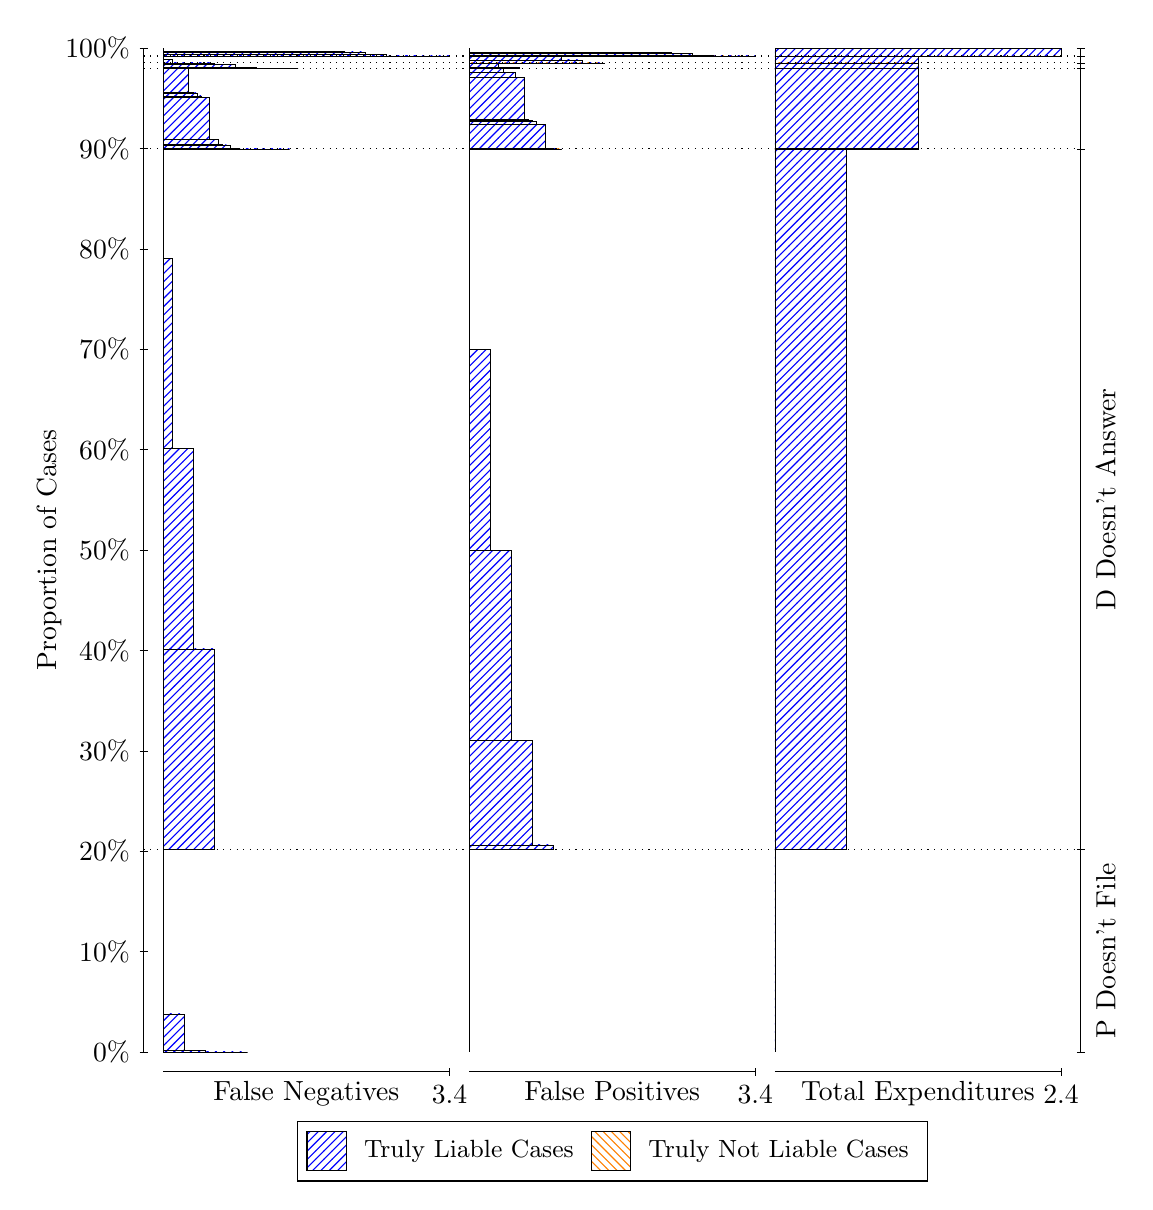
\begin{tikzpicture}
\draw[black, very thin] (1.5,1.75) -- (1.5,14.5);
\node[rotate=90, anchor=center] at (0.3, 8.125) {Proportion of Cases};
\draw[black, very thin] (1.45,1.75) -- (1.55,1.75);
\node[anchor=east] at (1.45, 1.75) {0\%};
\draw[black, very thin] (1.45,3.025) -- (1.55,3.025);
\node[anchor=east] at (1.45, 3.025) {10\%};
\draw[black, very thin] (1.45,4.3) -- (1.55,4.3);
\node[anchor=east] at (1.45, 4.3) {20\%};
\draw[black, very thin] (1.45,5.575) -- (1.55,5.575);
\node[anchor=east] at (1.45, 5.575) {30\%};
\draw[black, very thin] (1.45,6.85) -- (1.55,6.85);
\node[anchor=east] at (1.45, 6.85) {40\%};
\draw[black, very thin] (1.45,8.125) -- (1.55,8.125);
\node[anchor=east] at (1.45, 8.125) {50\%};
\draw[black, very thin] (1.45,9.4) -- (1.55,9.4);
\node[anchor=east] at (1.45, 9.4) {60\%};
\draw[black, very thin] (1.45,10.675) -- (1.55,10.675);
\node[anchor=east] at (1.45, 10.675) {70\%};
\draw[black, very thin] (1.45,11.95) -- (1.55,11.95);
\node[anchor=east] at (1.45, 11.95) {80\%};
\draw[black, very thin] (1.45,13.225) -- (1.55,13.225);
\node[anchor=east] at (1.45, 13.225) {90\%};
\draw[black, very thin] (1.45,14.5) -- (1.55,14.5);
\node[anchor=east] at (1.45, 14.5) {100\%};

\draw[black, very thin] (13.4,1.75) -- (13.4,14.5);
\draw[black, very thin] (13.35,1.75) -- (13.45,1.75);
\node[anchor=west] at (13.35, 1.75) {};
\draw[black, very thin] (13.35,4.3188) -- (13.45,4.3188);
\node[anchor=west] at (13.35, 4.3188) {};
\draw[black, very thin] (13.35,13.22) -- (13.45,13.22);
\node[anchor=west] at (13.35, 13.22) {};
\draw[black, very thin] (13.35,14.242) -- (13.45,14.242);
\node[anchor=west] at (13.35, 14.242) {};
\draw[black, very thin] (13.35,14.311) -- (13.45,14.311);
\node[anchor=west] at (13.35, 14.311) {};
\draw[black, very thin] (13.35,14.399) -- (13.45,14.399);
\node[anchor=west] at (13.35, 14.399) {};
\draw[black, very thin] (13.35,14.5) -- (13.45,14.5);
\node[anchor=west] at (13.35, 14.5) {};

\draw[black, very thin, pattern color=blue, pattern=north east lines] (1.75,1.75) rectangle (2.8186,1.75);
\draw[black, very thin, pattern color=blue, pattern=north east lines] (1.75,1.75) rectangle (2.5515,1.7501);
\draw[black, very thin, pattern color=blue, pattern=north east lines] (1.75,1.7501) rectangle (2.2843,1.768);
\draw[black, very thin, pattern color=blue, pattern=north east lines] (1.75,1.768) rectangle (2.0172,2.2325);
\draw[black, very thin, pattern color=orange, pattern=north west lines] (1.75,2.2325) rectangle (1.75,2.2325);
\draw[black, very thin, pattern color=blue, pattern=north east lines] (1.75,2.2325) rectangle (1.75,4.3188);
\draw[black, very thin, pattern color=blue, pattern=north east lines] (1.75,4.3188) rectangle (2.3912,6.8688);
\draw[black, very thin, pattern color=blue, pattern=north east lines] (1.75,6.8688) rectangle (2.124,9.4176);
\draw[black, very thin, pattern color=blue, pattern=north east lines] (1.75,9.4176) rectangle (1.8569,11.827);
\draw[black, very thin, pattern color=orange, pattern=north west lines] (1.75,11.827) rectangle (1.75,11.827);
\draw[black, very thin, pattern color=blue, pattern=north east lines] (1.75,11.827) rectangle (1.75,13.22);
\draw[black, very thin, pattern color=blue, pattern=north east lines] (1.75,13.22) rectangle (3.3529,13.22);
\draw[black, very thin, pattern color=blue, pattern=north east lines] (1.75,13.22) rectangle (3.2461,13.22);
\draw[black, very thin, pattern color=blue, pattern=north east lines] (1.75,13.22) rectangle (3.1392,13.22);
\draw[black, very thin, pattern color=blue, pattern=north east lines] (1.75,13.22) rectangle (3.0858,13.22);
\draw[black, very thin, pattern color=blue, pattern=north east lines] (1.75,13.22) rectangle (3.0324,13.22);
\draw[black, very thin, pattern color=blue, pattern=north east lines] (1.75,13.22) rectangle (2.9789,13.22);
\draw[black, very thin, pattern color=blue, pattern=north east lines] (1.75,13.22) rectangle (2.9255,13.22);
\draw[black, very thin, pattern color=blue, pattern=north east lines] (1.75,13.22) rectangle (2.8721,13.22);
\draw[black, very thin, pattern color=blue, pattern=north east lines] (1.75,13.22) rectangle (2.8186,13.22);
\draw[black, very thin, pattern color=blue, pattern=north east lines] (1.75,13.22) rectangle (2.7652,13.22);
\draw[black, very thin, pattern color=blue, pattern=north east lines] (1.75,13.22) rectangle (2.7118,13.222);
\draw[black, very thin, pattern color=blue, pattern=north east lines] (1.75,13.222) rectangle (2.6583,13.222);
\draw[black, very thin, pattern color=blue, pattern=north east lines] (1.75,13.222) rectangle (2.6049,13.268);
\draw[black, very thin, pattern color=blue, pattern=north east lines] (1.75,13.268) rectangle (2.5515,13.271);
\draw[black, very thin, pattern color=blue, pattern=north east lines] (1.75,13.271) rectangle (2.498,13.273);
\draw[black, very thin, pattern color=blue, pattern=north east lines] (1.75,13.273) rectangle (2.4446,13.336);
\draw[black, very thin, pattern color=blue, pattern=north east lines] (1.75,13.336) rectangle (2.3912,13.338);
\draw[black, very thin, pattern color=blue, pattern=north east lines] (1.75,13.338) rectangle (2.3377,13.874);
\draw[black, very thin, pattern color=blue, pattern=north east lines] (1.75,13.874) rectangle (2.2843,13.878);
\draw[black, very thin, pattern color=blue, pattern=north east lines] (1.75,13.878) rectangle (2.2309,13.892);
\draw[black, very thin, pattern color=blue, pattern=north east lines] (1.75,13.892) rectangle (2.1775,13.931);
\draw[black, very thin, pattern color=blue, pattern=north east lines] (1.75,13.931) rectangle (2.124,13.933);
\draw[black, very thin, pattern color=blue, pattern=north east lines] (1.75,13.933) rectangle (2.0706,14.241);
\draw[black, very thin, pattern color=blue, pattern=north east lines] (1.75,14.241) rectangle (1.9637,14.242);
\draw[black, very thin, pattern color=blue, pattern=north east lines] (1.75,14.242) rectangle (1.8569,14.242);
\draw[black, very thin, pattern color=orange, pattern=north west lines] (1.75,14.242) rectangle (1.75,14.242);
\draw[black, very thin, pattern color=blue, pattern=north east lines] (1.75,14.242) rectangle (3.4598,14.242);
\draw[black, very thin, pattern color=blue, pattern=north east lines] (1.75,14.242) rectangle (3.1926,14.242);
\draw[black, very thin, pattern color=blue, pattern=north east lines] (1.75,14.242) rectangle (2.9255,14.254);
\draw[black, very thin, pattern color=blue, pattern=north east lines] (1.75,14.254) rectangle (2.6583,14.296);
\draw[black, very thin, pattern color=blue, pattern=north east lines] (1.75,14.296) rectangle (2.3912,14.311);
\draw[black, very thin, pattern color=orange, pattern=north west lines] (1.75,14.311) rectangle (1.75,14.311);
\draw[black, very thin, pattern color=blue, pattern=north east lines] (1.75,14.311) rectangle (2.3912,14.311);
\draw[black, very thin, pattern color=blue, pattern=north east lines] (1.75,14.311) rectangle (2.124,14.312);
\draw[black, very thin, pattern color=blue, pattern=north east lines] (1.75,14.312) rectangle (1.8569,14.36);
\draw[black, very thin, pattern color=orange, pattern=north west lines] (1.75,14.36) rectangle (1.75,14.36);
\draw[black, very thin, pattern color=blue, pattern=north east lines] (1.75,14.36) rectangle (1.75,14.399);
\draw[black, very thin, pattern color=blue, pattern=north east lines] (1.75,14.399) rectangle (5.3833,14.399);
\draw[black, very thin, pattern color=blue, pattern=north east lines] (1.75,14.399) rectangle (5.1162,14.399);
\draw[black, very thin, pattern color=blue, pattern=north east lines] (1.75,14.399) rectangle (4.849,14.4);
\draw[black, very thin, pattern color=blue, pattern=north east lines] (1.75,14.4) rectangle (4.5819,14.415);
\draw[black, very thin, pattern color=blue, pattern=north east lines] (1.75,14.415) rectangle (4.3147,14.452);
\draw[black, very thin, pattern color=blue, pattern=north east lines] (1.75,14.452) rectangle (4.0475,14.453);
\draw[black, very thin, pattern color=blue, pattern=north east lines] (1.75,14.453) rectangle (3.7804,14.453);
\draw[black, very thin, pattern color=blue, pattern=north east lines] (1.75,14.453) rectangle (2.5515,14.453);
\draw[black, very thin, pattern color=blue, pattern=north east lines] (1.75,14.453) rectangle (2.2843,14.453);
\draw[black, very thin, pattern color=blue, pattern=north east lines] (1.75,14.453) rectangle (2.0172,14.453);
\draw[black, very thin, pattern color=orange, pattern=north west lines] (1.75,14.453) rectangle (1.75,14.453);
\draw[black, very thin, pattern color=blue, pattern=north east lines] (1.75,14.453) rectangle (1.75,14.5);
\draw[black, very thin, pattern color=orange, pattern=north west lines] (5.6333,1.75) rectangle (5.6333,1.75);
\draw[black, very thin, pattern color=blue, pattern=north east lines] (5.6333,1.75) rectangle (5.6333,4.3188);
\draw[black, very thin, pattern color=orange, pattern=north west lines] (5.6333,4.3188) rectangle (6.702,4.3188);
\draw[black, very thin, pattern color=blue, pattern=north east lines] (5.6333,4.3188) rectangle (6.702,4.3804);
\draw[black, very thin, pattern color=blue, pattern=north east lines] (5.6333,4.3804) rectangle (6.4348,5.7118);
\draw[black, very thin, pattern color=blue, pattern=north east lines] (5.6333,5.7118) rectangle (6.1676,8.1216);
\draw[black, very thin, pattern color=blue, pattern=north east lines] (5.6333,8.1216) rectangle (5.9005,10.67);
\draw[black, very thin, pattern color=blue, pattern=north east lines] (5.6333,10.67) rectangle (5.6333,13.22);
\draw[black, very thin, pattern color=orange, pattern=north west lines] (5.6333,13.22) rectangle (6.8088,13.22);
\draw[black, very thin, pattern color=blue, pattern=north east lines] (5.6333,13.22) rectangle (6.8088,13.22);
\draw[black, very thin, pattern color=orange, pattern=north west lines] (5.6333,13.22) rectangle (6.702,13.22);
\draw[black, very thin, pattern color=blue, pattern=north east lines] (5.6333,13.22) rectangle (6.702,13.221);
\draw[black, very thin, pattern color=orange, pattern=north west lines] (5.6333,13.221) rectangle (6.5951,13.221);
\draw[black, very thin, pattern color=blue, pattern=north east lines] (5.6333,13.221) rectangle (6.5951,13.529);
\draw[black, very thin, pattern color=blue, pattern=north east lines] (5.6333,13.529) rectangle (6.5417,13.531);
\draw[black, very thin, pattern color=orange, pattern=north west lines] (5.6333,13.531) rectangle (6.4882,13.531);
\draw[black, very thin, pattern color=blue, pattern=north east lines] (5.6333,13.531) rectangle (6.4882,13.571);
\draw[black, very thin, pattern color=blue, pattern=north east lines] (5.6333,13.571) rectangle (6.4348,13.585);
\draw[black, very thin, pattern color=orange, pattern=north west lines] (5.6333,13.585) rectangle (6.3814,13.585);
\draw[black, very thin, pattern color=blue, pattern=north east lines] (5.6333,13.585) rectangle (6.3814,13.589);
\draw[black, very thin, pattern color=blue, pattern=north east lines] (5.6333,13.589) rectangle (6.3279,14.125);
\draw[black, very thin, pattern color=blue, pattern=north east lines] (5.6333,14.125) rectangle (6.2745,14.127);
\draw[black, very thin, pattern color=blue, pattern=north east lines] (5.6333,14.127) rectangle (6.2211,14.19);
\draw[black, very thin, pattern color=blue, pattern=north east lines] (5.6333,14.19) rectangle (6.1676,14.192);
\draw[black, very thin, pattern color=blue, pattern=north east lines] (5.6333,14.192) rectangle (6.1142,14.195);
\draw[black, very thin, pattern color=blue, pattern=north east lines] (5.6333,14.195) rectangle (6.0608,14.24);
\draw[black, very thin, pattern color=blue, pattern=north east lines] (5.6333,14.24) rectangle (6.0074,14.24);
\draw[black, very thin, pattern color=blue, pattern=north east lines] (5.6333,14.24) rectangle (5.9539,14.242);
\draw[black, very thin, pattern color=blue, pattern=north east lines] (5.6333,14.242) rectangle (5.9005,14.242);
\draw[black, very thin, pattern color=blue, pattern=north east lines] (5.6333,14.242) rectangle (5.8471,14.242);
\draw[black, very thin, pattern color=blue, pattern=north east lines] (5.6333,14.242) rectangle (5.7936,14.242);
\draw[black, very thin, pattern color=blue, pattern=north east lines] (5.6333,14.242) rectangle (5.7402,14.242);
\draw[black, very thin, pattern color=blue, pattern=north east lines] (5.6333,14.242) rectangle (5.6868,14.242);
\draw[black, very thin, pattern color=blue, pattern=north east lines] (5.6333,14.242) rectangle (5.6333,14.242);
\draw[black, very thin, pattern color=orange, pattern=north west lines] (5.6333,14.242) rectangle (6.2745,14.242);
\draw[black, very thin, pattern color=blue, pattern=north east lines] (5.6333,14.242) rectangle (6.2745,14.258);
\draw[black, very thin, pattern color=blue, pattern=north east lines] (5.6333,14.258) rectangle (6.0074,14.3);
\draw[black, very thin, pattern color=blue, pattern=north east lines] (5.6333,14.3) rectangle (5.7402,14.311);
\draw[black, very thin, pattern color=blue, pattern=north east lines] (5.6333,14.311) rectangle (5.6333,14.311);
\draw[black, very thin, pattern color=orange, pattern=north west lines] (5.6333,14.311) rectangle (7.3431,14.311);
\draw[black, very thin, pattern color=blue, pattern=north east lines] (5.6333,14.311) rectangle (7.3431,14.312);
\draw[black, very thin, pattern color=blue, pattern=north east lines] (5.6333,14.312) rectangle (7.076,14.35);
\draw[black, very thin, pattern color=blue, pattern=north east lines] (5.6333,14.35) rectangle (6.8088,14.399);
\draw[black, very thin, pattern color=blue, pattern=north east lines] (5.6333,14.399) rectangle (6.5417,14.399);
\draw[black, very thin, pattern color=blue, pattern=north east lines] (5.6333,14.399) rectangle (6.2745,14.399);
\draw[black, very thin, pattern color=orange, pattern=north west lines] (5.6333,14.399) rectangle (9.2667,14.399);
\draw[black, very thin, pattern color=blue, pattern=north east lines] (5.6333,14.399) rectangle (9.2667,14.399);
\draw[black, very thin, pattern color=orange, pattern=north west lines] (5.6333,14.399) rectangle (8.9995,14.399);
\draw[black, very thin, pattern color=blue, pattern=north east lines] (5.6333,14.399) rectangle (8.9995,14.399);
\draw[black, very thin, pattern color=orange, pattern=north west lines] (5.6333,14.399) rectangle (8.7324,14.399);
\draw[black, very thin, pattern color=blue, pattern=north east lines] (5.6333,14.399) rectangle (8.7324,14.402);
\draw[black, very thin, pattern color=orange, pattern=north west lines] (5.6333,14.402) rectangle (8.4652,14.402);
\draw[black, very thin, pattern color=blue, pattern=north east lines] (5.6333,14.402) rectangle (8.4652,14.428);
\draw[black, very thin, pattern color=blue, pattern=north east lines] (5.6333,14.428) rectangle (8.198,14.447);
\draw[black, very thin, pattern color=blue, pattern=north east lines] (5.6333,14.447) rectangle (7.9309,14.447);
\draw[black, very thin, pattern color=blue, pattern=north east lines] (5.6333,14.447) rectangle (7.6637,14.447);
\draw[black, very thin, pattern color=blue, pattern=north east lines] (5.6333,14.447) rectangle (7.3966,14.447);
\draw[black, very thin, pattern color=orange, pattern=north west lines] (5.6333,14.447) rectangle (6.1676,14.447);
\draw[black, very thin, pattern color=blue, pattern=north east lines] (5.6333,14.447) rectangle (6.1676,14.447);
\draw[black, very thin, pattern color=orange, pattern=north west lines] (5.6333,14.447) rectangle (5.9005,14.447);
\draw[black, very thin, pattern color=blue, pattern=north east lines] (5.6333,14.447) rectangle (5.9005,14.447);
\draw[black, very thin, pattern color=orange, pattern=north west lines] (5.6333,14.447) rectangle (5.6333,14.447);
\draw[black, very thin, pattern color=blue, pattern=north east lines] (5.6333,14.447) rectangle (5.6333,14.5);
\draw[black, very thin, pattern color=orange, pattern=north west lines] (9.5167,1.75) rectangle (9.5167,1.75);
\draw[black, very thin, pattern color=blue, pattern=north east lines] (9.5167,1.75) rectangle (9.5167,4.3188);
\draw[black, very thin, pattern color=orange, pattern=north west lines] (9.5167,4.3188) rectangle (10.425,4.3188);
\draw[black, very thin, pattern color=blue, pattern=north east lines] (9.5167,4.3188) rectangle (10.425,13.22);
\draw[black, very thin, pattern color=orange, pattern=north west lines] (9.5167,13.22) rectangle (11.333,13.22);
\draw[black, very thin, pattern color=blue, pattern=north east lines] (9.5167,13.22) rectangle (11.333,13.224);
\draw[black, very thin, pattern color=orange, pattern=north west lines] (9.5167,13.224) rectangle (11.333,13.224);
\draw[black, very thin, pattern color=blue, pattern=north east lines] (9.5167,13.224) rectangle (11.333,14.242);
\draw[black, very thin, pattern color=orange, pattern=north west lines] (9.5167,14.242) rectangle (11.333,14.242);
\draw[black, very thin, pattern color=blue, pattern=north east lines] (9.5167,14.242) rectangle (11.333,14.311);
\draw[black, very thin, pattern color=orange, pattern=north west lines] (9.5167,14.311) rectangle (11.333,14.311);
\draw[black, very thin, pattern color=blue, pattern=north east lines] (9.5167,14.311) rectangle (11.333,14.399);
\draw[black, very thin, pattern color=orange, pattern=north west lines] (9.5167,14.399) rectangle (13.15,14.399);
\draw[black, very thin, pattern color=blue, pattern=north east lines] (9.5167,14.399) rectangle (13.15,14.5);
\draw[black, dotted] (1.5,4.3188) -- (13.4,4.3188);
\draw[black, dotted] (1.5,13.22) -- (13.4,13.22);
\draw[black, dotted] (1.5,14.242) -- (13.4,14.242);
\draw[black, dotted] (1.5,14.311) -- (13.4,14.311);
\draw[black, dotted] (1.5,14.399) -- (13.4,14.399);
\draw[black, very thin] (1.75,1.5) -- (5.3833,1.5);
\node[anchor=north] at (3.5667, 1.5) {False Negatives};
\draw[black, very thin] (5.3833,1.45) -- (5.3833,1.55);
\node[anchor=north] at (5.3833, 1.45) {3.4};

\draw[black, very thin] (5.6333,1.5) -- (9.2667,1.5);
\node[anchor=north] at (7.45, 1.5) {False Positives};
\draw[black, very thin] (9.2667,1.45) -- (9.2667,1.55);
\node[anchor=north] at (9.2667, 1.45) {3.4};

\draw[black, very thin] (9.5167,1.5) -- (13.15,1.5);
\node[anchor=north] at (11.333, 1.5) {Total Expenditures};
\draw[black, very thin] (13.15,1.45) -- (13.15,1.55);
\node[anchor=north] at (13.15, 1.45) {2.4};

\node[black, centered, rotate=90] at (13.72, 3.0344) {P Doesn't File};
\node[black, centered, rotate=90] at (13.72, 8.7696) {D Doesn't Answer};





\draw (7.449999999999999,1.5) node[draw=none] (baseCoordinate) {};
\begin{scope}[align=center]
        \matrix[scale=0.5, draw=black, below=0.5cm of baseCoordinate, nodes={draw}, column sep=0.1cm]{
            \node[rectangle, draw, minimum width=0.5cm, minimum height=0.5cm, pattern=north east lines, pattern color=blue] {}; &
            \node[draw=none, font=\small] (B) {Truly Liable Cases}; &
            \node[rectangle, draw, minimum width=0.5cm, minimum height=0.5cm, pattern=north west lines, pattern color=orange] {}; &
            \node[draw=none, font=\small] (B) {Truly Not Liable Cases}; \\
            };
\end{scope}

\end{tikzpicture}
\end{document}